\section{Lab: Xv6 and Unix utilities}
\subsection{实验目的}

本实验旨在熟悉xv6操作系统及其系统调用。通过本次实验,我将学习如何在xv6环境中设置并运行操作系统,理解并实现基本的UNIX实用程序。这包括启动xv6、获取并管理源代码、编译和运行操作系统、以及实现和测试具体的系统调用和应用程序。本实验将帮助深入理解操作系统的运行机制和开发流程,为后续更复杂的操作系统编程打下坚实基础。

具体将实现以下程序:
\begin{itemize}
    \item sleep程序:编写一个xv6版本的sleep程序,使其根据用户指定的ticks暂停。
    \item pingpong程序:编写一个使用管道和fork系统调用在父子进程间传递字节的程序。
    \item primes程序:编写一个基于管道的并发素数筛选程序,将数值在进程间传递并筛选素数。
    \item find程序:编写一个简化版的find程序,遍历目录树查找特定文件名。
    \item xargs程序:编写一个简化版的xargs程序,从标准输入读取行并为每行运行一个命令。
\end{itemize}

在实现和测试这些系统调用的过程中,我们将深入理解操作系统的内部机制,并掌握如何在用户程序中调用这些功能。
\subsection{实验步骤}
\subsubsection{运行xv6}
\begin{enumerate}
    \item 利用以下指令获取Lab xv6源代码,查看util分支。
          \begin{lstlisting}
    $ git clone git://g.csail.mit.edu/xv6-labs-2021
    $ cd xv6-labs-2021
    $ git checkout util
        \end{lstlisting}
    \item 输入make qemu命令构建并运行xv6。
          \begin{lstlisting}
    $ make qemu
    
    ...

    xv6 kernel is booting

    hart 2 starting
    hart 1 starting
    init: starting sh
        \end{lstlisting}
\end{enumerate}

\subsubsection{实现sleep}

\begin{enumerate}
    \item 根据题目提示,可以实现如下代码:
          \begin{lstlisting}[language=c, title=sleep.c]
    #include "kernel/types.h"   // 包含内核类型定义
    #include "user/user.h"      // 包含用户模式下的库函数

    int main(int argc, char *argv[])
    {
        // 检查命令行参数是否等于2,即程序名和等待时间参数
        if (argc != 2)
        {
            fprintf(2, "Error: Parameters Error\n"); // 打印错误信息
            exit(1); // 退出程序,返回状态码1
        }

        sleep(atoi(argv[1])); // 调用 sleep 函数,等待指定的秒数

        exit(0); // 程序正常退出,返回状态码0
    }
        \end{lstlisting}
    \item 在 Makefile 文件中的UPROGS加上\$U/\_sleep\textbackslash 后利用make qemu命令编译启动xv6操作系统;
    \item 在xv6命令行中运行sleep,程序将暂停执行一段指定的时间:
          \begin{lstlisting}
    $ sleep 10
        \end{lstlisting}
\end{enumerate}

\subsubsection{实现pingpong}

\begin{enumerate}
    \item 首先创建两条管道和用于储存数据的缓冲区。
          \begin{lstlisting}[language=c,title=初始化管道和缓冲区]
    int fd1[2];
    int fd2[2];

    pipe(fd1);
    pipe(fd2);

    char buffer[16];
            \end{lstlisting}
    \item 利用fork()创建子进程。
          \begin{lstlisting}[language=c,title=fork()函数]
    if (fork() != 0)
    {
        // 父线程执行的代码...
    }
    else
    {
        // 子线程执行的代码...
    }
            \end{lstlisting}
    \item 在父进程中发送“ping”并接收“pong”。
          \begin{lstlisting}[language=c, title=父进程]
    // 父线程执行的代码
    write(fd1[1], "ping", strlen("ping"));
    read(fd2[0], buffer, 4);
    printf("%d: received %s\n", getpid(), buffer);
    \end{lstlisting}
    \item 在子进程中发送“pong”并接收“ping”。
          \begin{lstlisting}[language=c, title=子进程]
    // 子线程执行的代码
    read(fd1[0], buffer, 4);
    printf("%d: received %s\n", getpid(), buffer);
    write(fd2[1], "pong", strlen("pong"));
    \end{lstlisting}
    \item 把程序写在pingpong.c中,用同样的方法在xv6中运行程序,可以观察到父子进程分别输出的结果。
          \begin{lstlisting}
    $ pingpong
    5: received ping
    4: received pong
    \end{lstlisting}
\end{enumerate}

\subsubsection{实现 prime}
\begin{enumerate}
    \begin{figure}[h]
        \centering
        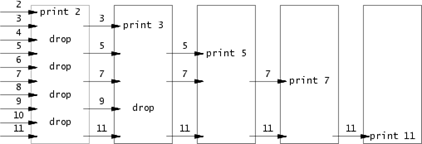
\includegraphics[width=\linewidth]{pics/图片1.png}
        \caption{primes程序原理}
        \label{fig:primes}
    \end{figure}
    \item 首先了解程序的原理。原理示意见图\ref{fig:primes}。程序通过递归创建进程和使用管道通信的方式,逐步筛选出素数。每个进程从管道中读取数值,将第一个数识别为素数,并过滤掉其倍数,然后将剩余的数传递给下一个进程继续处理,从而并发地筛选出所有素数。
    \item 把输出质数,创建子进程并向其传送数据的过程整合为一个递归函数。要注意文件描述符的回收,防止资源超限。
          \begin{lstlisting}[language=c, title=new\_prime\_proc函数的实现]
    void new_prime_proc(int *old_pipe)
    {
        close(old_pipe[1]); // 关闭旧管道的写端

        int first_num;
        // 从旧管道中读取第一个数,如果读取失败则退出
        if (!read(old_pipe[0], &first_num, sizeof(first_num)))
        {
            close(old_pipe[0]); // 关闭旧管道的读端
            exit(0);            // 退出进程
        }

        fprintf(1, "prime %d\n", first_num); // 打印第一个数,即当前的素数

        int new_pipe[2];
        pipe(new_pipe); // 创建新管道

        int p_id = fork(); // 创建子进程
        if (p_id == 0)
            new_prime_proc(new_pipe); // 子进程递归调用处理新管道
        else
        {
            int t;
            // 在父进程中,从旧管道中读取数,如果不是first_num的倍数则写入新管道
            while (read(old_pipe[0], &t, sizeof(t)))
            {
                if (t % first_num != 0)
                {
                    write(new_pipe[1], &t, sizeof(t));
                }
            }

            close(old_pipe[0]); // 关闭旧管道的读端
            close(new_pipe[0]); // 关闭新管道的读端
            close(new_pipe[1]); // 关闭新管道的写端

            wait((int *)0); // 等待子进程结束
        }
    }
    \end{lstlisting}
    \item 在主函数中将2~35写入管道,调用递归函数。
          \begin{lstlisting}[language=c, title=main()函数的实现]
    int main()
    {
        int p[2];
        pipe(p); // 创建管道
        int i;
        // 向管道中写入从2到35的所有数
        for (i = 2; i <= 35; i++)
            write(p[1], &i, sizeof(i));
        new_prime_proc(p); // 调用处理函数处理管道中的数
    
        exit(0); // 退出程序
    }
    \end{lstlisting}
    \item 把程序写在primes.c中,运行程序得到结果。
          \begin{lstlisting}
    $ primes
    prime 2
    prime 3
    ...
    prime 31
    \end{lstlisting}
\end{enumerate}

\subsubsection{实现 find}

\begin{enumerate}
    \item 首先,仿照ls.c实现一个辅助函数char*fmtname(char *path),把路径末尾的文件名提取出来,实现过程略。
    \item 利用深度优先搜索的思想,实现一个find函数递归寻找文件。
          \begin{lstlisting}[language=c, title=find函数的实现]
    void find(char *path, char *target)
    {
        char buf[512], *p;
        int fd;
        struct dirent de;
        struct stat st;

        // 打开指定路径的文件或目录
        if ((fd = open(path, 0)) < 0)
        {
            fprintf(2, "find: cannot open %s\n", path);
            return;
        }

        // 获取文件或目录的状态信息
        if (fstat(fd, &st) < 0)
        {
            fprintf(2, "find1: cannot stat %s\n", path); 
            close(fd);
            return;
        }

        // 根据文件或目录的类型进行处理
        switch (st.type)
        {
        case T_FILE:
            // 如果是文件,比较文件名是否与目标名称相同
            if (strcmp(target, path2name(path)) == 0)
            {
                printf("%s\n", path); // 输出文件路径
            }

            break;
        case T_DIR:
            // 如果是目录,检查路径长度是否超出缓冲区范围
            if (strlen(path) + 1 + DIRSIZ + 1 > sizeof buf)
            {
                printf("find: path too long\n"); // 输出错误信息,路径过长
                break;
            }
            strcpy(buf, path); // 将路径复制到缓冲区
            p = buf + strlen(buf);
            *p++ = '/';

            // 遍历目录中的每个文件或子目录
            while (read(fd, &de, sizeof(de)) == sizeof(de))
            {
                if (de.inum == 0)
                    continue; // 跳过空目录项

                memmove(p, de.name, DIRSIZ); // 将文件或目录名复制到缓冲区末尾
                p[DIRSIZ] = 0;               // 添加字符串结束符

                // 获取文件或目录的状态信息
                if (stat(buf, &st) < 0)
                {
                    // 输出错误信息,无法获取文件或目录的状态信息
                    printf("find2: cannot stat %s\n", buf); 
                    continue;
                }

                // 排除当前目录和上级目录的特殊情况
                if (strlen(de.name) == 1 && de.name[0] == '.')
                    continue;
                if (strlen(de.name) == 2 
                && de.name[0] == '.' 
                && de.name[1] == '.')
                    continue;
                find(buf, target); // 递归调用查找函数,继续查找子目录
            }
            break;
        }

        close(fd); // 关闭文件或目录
    }
    \end{lstlisting}
    \item 在主函数中调用find函数。
    \item 将程序写在find.c中,运行程序得到结果。
          \begin{lstlisting}
    $ find . b
    ./a/b
    ./b
    \end{lstlisting}
\end{enumerate}

\subsubsection{实现 xargs}
\begin{enumerate}
    \item 首先初始化一些变量。
          \begin{lstlisting}[language=c, title=初始化]
    int i;
    int arg_count = 0;  // 参数数量计数器
    char *args[MAXARG]; // 参数数组,最大长度为MAXARG
    int initial_arg_count = arg_count; // 存储初始参数数量的位置
    
    int line_index = 0; // 当前行的索引
    char input_char;                   // 用于读取字符
    char *current_line;                // 指向当前处理的行
    char line_buffer[512];             // 临时存储字符串的缓冲区
    current_line = line_buffer;

    // 将命令行参数复制到参数数组args中
    for (i = 1; i < argc; ++i)
    {
        args[arg_count++] = argv[i];
    }
    \end{lstlisting}
    \item 循环处理读取的字符。
          \begin{lstlisting}[language=c, title=输入处理循环]
    while (read(0, &input_char, 1) > 0)
    {
        // 对输入字符的操作...
    }
    \end{lstlisting}
    \item 循环中的字符处理:\begin{itemize}
              \item 对于普通字符,将其加入到当前行末尾;
              \item 遇到空格,表示一个参数已经结束,将参数添加到参数列表之中;
                    \begin{lstlisting}[language=c, title=空格的处理]
    current_line[line_index] = '\0';  // 添加字符串结束符
    line_index = 0;                   // 重置索引
    args[arg_count++] = current_line; // 将当前单词添加到参数数组
    char line_buffer[512];            // 重新分配缓冲区
    current_line = line_buffer;
        \end{lstlisting}
              \item 遇到回车,表示一行结束,将最后一个参数加入参数列表之中并执行命令。
                    \begin{lstlisting}[language=c, title=回车的处理]
    // 处理换行符,将当前行作为参数
    current_line[line_index] = '\0'; // 添加字符串结束符
    line_index = 0;                  // 重置索引

    args[arg_count++] = current_line; // 将当前行添加到参数数组
    args[arg_count] = 0;              // 设置参数数组的结束标志

    if (fork()) // 创建子进程
    {
        wait(0);                       // 父进程等待子进程结束
        arg_count = initial_arg_count; // 重置参数数量
    }
    else
    {
        exec(argv[1], args); // 子进程执行命令
    }
            \end{lstlisting}
          \end{itemize}
    \item 将程序写入xargs.c中,运行程序得到结果。
          \begin{lstlisting}
    $ echo hello too | xargs echo bye 
    bye hello too
    \end{lstlisting}
\end{enumerate}

\subsection{评测结果}

利用grade-lab-util脚本评测,得到结果见图\ref{fig:util}
\begin{figure}[h]
    \centering
    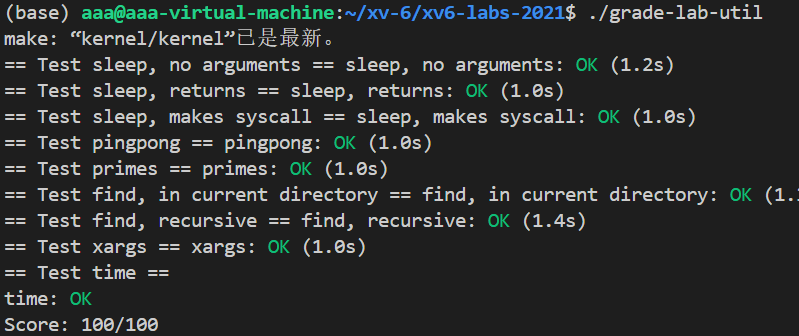
\includegraphics[width=\linewidth]{pics/util评测结果.png}
    \caption{评测结果}
    \label{fig:util}
\end{figure}

\subsection{实验小结}
本实验中我初步了解了xv6这个操作系统的基本结构。了解了其利用qemu模拟器运行、编程的基本方法。本实验中需要实现的多为基本的系统功能,让我对Unix操作系统有了更深入的了解。

此外primes是我认为这里面最难的程序。首先,理解这个程序的实现原理就花费了我不少时间。在之后实现这个程序的过程之中,我在处理管道、父子进程的关系的时候遇到了一些困难。不过最后我还是成功实现了程序,这对我理解管道、进程并行有很大的帮助。